\documentclass[../main.tex]{subfiles}

\begin{document}

\problem{2}

Consider the problem of two steady, uniform, and incompressible fluid jets colliding at right angles as shown to form a common jet at an angle \(\theta\). 
The pressure everywhere is \(p_{atm}\), and gravity/shear stress can be safely neglected. 
The control volume is given by the dashed lines.
Write out, simplify (stating your assumptions), and solve the continuity equation and relevant momentum equations. 
Find the angle \(\theta\) in terms of the flow properties \(u_1, \dot{m}_1, v_2, \ \textrm{and} \ \dot{m}_2\) of the two jets (where \(\dot{m}\) is the mass flowrate). 
State your assumptions.

\begin{figure}[ht]
    \centering
    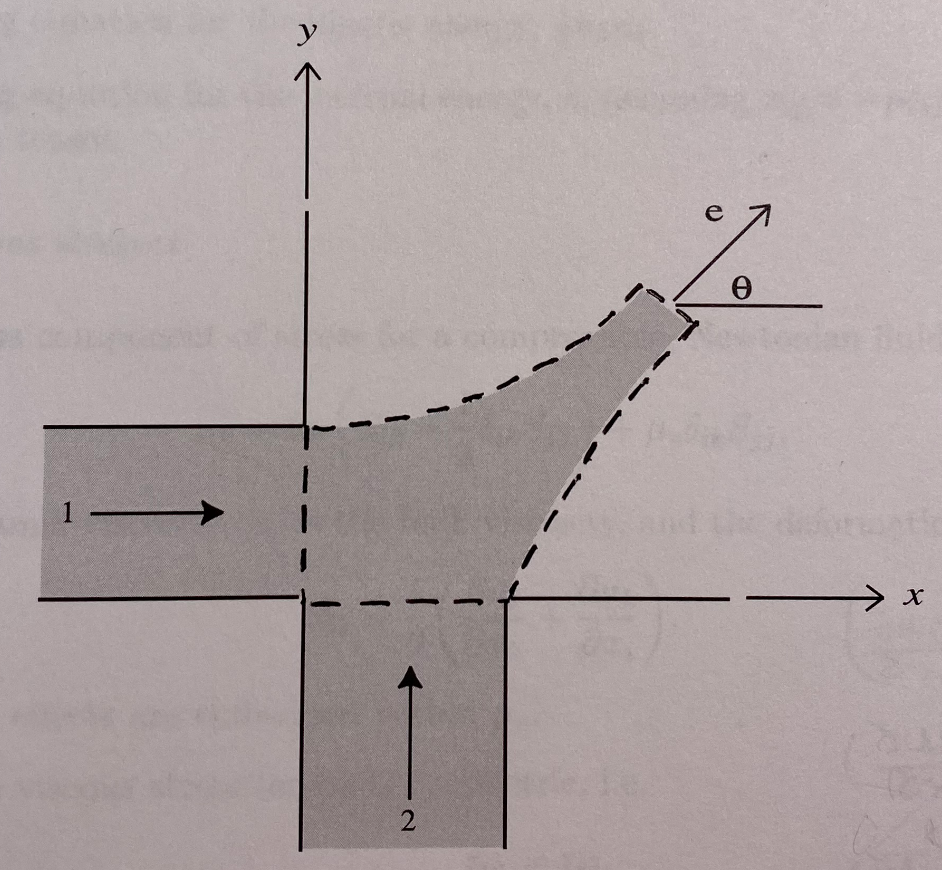
\includegraphics[scale=0.5]{images/problem2_diagram.png}
\end{figure}

\givens{}
\(u_1, \dot{m}_1, v_2, \dot{m}_2, \theta, p_{atm}\)

\assumptions{}
Steady, uniform, incompressible flow. 
Gravity and shear stress can be ignored. 
Pressure everywhere is $P_{atm}$.
Jets collide at a right angle.
All flow velocities are normal to inlets/outlets.

\solution{}
The full integral form of the conservation of mass equation is given by

\begin{equation*}
    \frac{\dd (m)_{sys}}{\dd t} = %
    \pdv{t} \int_{CV} \rho \dd \volume +%
    \int_{CS} \rho \left({\vec{V} \cdot \hat{\mathbf{n}}}\right) \dd A
    = 0
\end{equation*}

The assumption of steady flow removes the time-dependency of the continuity equation:

\begin{equation*}
    \cancelto{0}{\pdv{t} \int_{CV} \rho \dd \volume} +%
    \int_{CS} \rho \left({\vec{V} \cdot \hat{\mathbf{n}}}\right) \dd A
    = 0
\end{equation*}

\begin{equation*}
    \int_{CS} \rho \left({\vec{V} \cdot \hat{\mathbf{n}}}\right) \dd A
    = 0
\end{equation*}

The assumption of uniform flow removes the spatial dependence of the integrand:

\begin{equation*}
    \rho \left({\vec{V} \cdot \hat{\mathbf{n}}}\right) \int_{CS} \dd A
    = 0
\end{equation*}

This results in the following expression evaluated at every CS:

\begin{equation*}
    \left. \rho \left({\vec{V} \cdot \hat{\mathbf{n}}}\right) A \right|_{CS}
    = 0
\end{equation*}

The assumption of incompressibility implies that $\rho$ is constant throughout the flow and the same at every CS, and can therefore be divided out.

\begin{equation*}
    \left. \left({\vec{V} \cdot \hat{\mathbf{n}}}\right) A \right|_{CS}
    = 0
\end{equation*}

Recalling that \(\left({\vec{V} \cdot \hat{\mathbf{n}}}\right)\) can be expressed as \({-\lvert{\vec{V}_n}\rvert}\) for influx and \({+\lvert{\vec{V}_n}\rvert}\) for outflux, we rewrite the simplified form of the continuity equation in terms of influx and outflux:

\begin{equation*}
    \sum_{outflux} {\lvert{\vec{V}_n}\rvert A} -%
    \sum_{influx}  {\lvert{\vec{V}_n}\rvert A} = 0
\end{equation*}

\begin{equation*}
    \sum_{outflux} {\lvert{\vec{V}_n}\rvert A} = %
    \sum_{influx}  {\lvert{\vec{V}_n}\rvert A}
\end{equation*}

The sum of all mass influx terms must be equal to the sum of all outflux terms to satisfy continuity.

Examining our problem, with inlet control surfaces 1 and 2 and outlet control surface $e$, we apply the simplified form of continuity to yield:

\[
    V_1 A_1 + V_2 A_2 = V_e A_e  
\]

where $V_e$ represents the velocity in the exit direction.

Multiplying through by density yields an expression in terms of mass flow rate:

\[
    \rho V_1 A_1 + \rho V_2 A_2 = \rho V_e A_e
\]

\[
    \dot{m}_1 + \dot{m}_2 = \dot{m}_e
\]

The full integral form of the conservation of momentum equation is given by

\begin{equation*}
    \frac{\dd (m\vec{V})_{sys}}{\dd t} = %
    \pdv{t} \int_{CV} \rho \vec{V} \dd \volume +%
    \int_{CS} \rho \vec{V} \left({\vec{V} \cdot \hat{\mathbf{n}}}\right) \dd A =%
    \sum{\vec{F}_{CV}}
\end{equation*}

This is a vector equation that can be decomposed into its \(x,\, y, \, \textrm{and} \ z\) components as shown below:

\begin{align*}
    \pdv{t} \int_{CV} \rho \vec{u} \dd \volume +%
    \int_{CS} \rho \vec{u} \left({\vec{V} \cdot \hat{\mathbf{n}}}\right) \dd A &=%
    \sum{\vec{F}_{CV_x}}\\
    \pdv{t} \int_{CV} \rho \vec{v} \dd \volume +%
    \int_{CS} \rho \vec{v} \left({\vec{V} \cdot \hat{\mathbf{n}}}\right) \dd A &=%
    \sum{\vec{F}_{CV_y}}\\
    \pdv{t} \int_{CV} \rho \vec{w} \dd \volume +%
    \int_{CS} \rho \vec{w} \left({\vec{V} \cdot \hat{\mathbf{n}}}\right) \dd A &=%
    \sum{\vec{F}_{CV_z}}
\end{align*}

This problem is 2-dimensional in \(x \, \textrm{and} \, y\), so we can safely ignore the \(z\) component.
Applying our assumptions and observations to the momentum equation greatly simplifies their forms. 
\par
By applying the steady flow assumption, the time-dependency of the equations disappears:

\begin{align*}
    \cancelto{0}{\pdv{t} \int_{CV} \rho \vec{u} \dd \volume} +%
    \int_{CS} \rho \vec{u} \left({\vec{V} \cdot \hat{\mathbf{n}}}\right) \dd A &=%
    \sum{\vec{F}_{CV_x}}\\
    \cancelto{0}{\pdv{t} \int_{CV} \rho \vec{v} \dd \volume} +%
    \int_{CS} \rho \vec{v} \left({\vec{V} \cdot \hat{\mathbf{n}}}\right) \dd A &=%
    \sum{\vec{F}_{CV_y}}
\end{align*}

Next, the uniform flow assumption allows us to remove the integrand from the integral as they are invariant over the control surface, though the terms must still be evaluated at each CS>

\begin{align*}
    \left. \left( \rho \vec{u} \left({\vec{V} \cdot \hat{\mathbf{n}}}\right) \int_{CS} \dd A \right) \right|_{CS} &=%
    \sum{\vec{F}_{CV_x}}\\
    \left. \left( \rho \vec{v} \left({\vec{V} \cdot \hat{\mathbf{n}}}\right) \int_{CS}  \dd A \right) \right|_{CS} &=%
    \sum{\vec{F}_{CV_y}}
\end{align*}

The integral is now simple, and becomes \(A\), the area of each CS that the equation is evaluated upon.

\begin{align*}
    \left. \left( \rho \vec{u} \left({\vec{V} \cdot \hat{\mathbf{n}}}\right) A \right) \right|_{CS} &=%
    \sum{\vec{F}_{CV_x}}\\
    \left. \left( \rho \vec{v} \left({\vec{V} \cdot \hat{\mathbf{n}}}\right) A \right) \right|_{CS} &=%
    \sum{\vec{F}_{CV_y}}
\end{align*}

The assumption of normal flow velocity at each inlet/outlet allows us to replace \(\left({\vec{V} \cdot \hat{\mathbf{n}}}\right)\) with \(\lvert\vec{V}\rvert\).
\textit{Note: the simplification of the dot product removes a polarity on the velocity term. For inlets, the entire term is negative, and for outlets, it will be positive.}

\begin{align*}
    \left. \left( \rho \vec{u} \lvert\vec{V}\rvert  A \right) \right|_{CS} &=%
    \sum{\vec{F}_{CV_x}}\\
    \left. \left( \rho \vec{v} \lvert\vec{V}\rvert  A \right) \right|_{CS} &=%
    \sum{\vec{F}_{CV_y}}
\end{align*}

The RHS of each equation can be defined by evaluating the forces that act on the control volume.
Our assumptions explicitly disregard gravity (body force) and shear stress (surface force).
The CV does not have rigid walls or supports, therefore we can ignore reaction forces.
The final remaining component is pressure, a surface force.
We assume that the pressure on each CS is \(P_{atm}\), therefore there is no net pressure differential acting on the CV.
With these assumptions and observations, we conclude that the net force in both \(x \, \textrm{and} \, y\) is 0.

\begin{align*}
    \left. \left( \rho \vec{u} \lvert\vec{V}\rvert A \right) \right|_{CS} &=%
    0\\
    \left. \left( \rho \vec{v} \lvert\vec{V}\rvert A \right) \right|_{CS} &=%
    0
\end{align*}

We now evaluate the momentum equation in the \(x \, \textrm{and} \, y\) at each CS, beginning with \(x\), remembering that inlets are negative and outlets are positive.

\[
  \rho_e u_e \lvert\vec{V}_e\rvert A_e - \rho_1 u_1^2 A_1 = 0
\]

We recognize that \(u_e\) can be recast as \(V_e \cos \theta\).

\[
  \rho_e \left({V_e \cos \theta}\right) \lvert\vec{V}_e\rvert A_e - \rho_1 u_1^2 A_1 = 0
\]

The momentum equation in the \(y\) direction follows the same logic.

\[
    \rho_e \left({V_e \sin \theta}\right) \lvert\vec{V}_e\rvert A_e - \rho_2 v_v^2 A_2 = 0
\]

%%%%%%%%%%%%

We now recast the momentum equations in terms of mass flow rates found from the continuity equation:

\begin{align*}
    \dot{m}_e V_e \cos \theta - \dot{m}_1 u_1 &= 0\\
    \dot{m}_e V_e \sin \theta - \dot{m}_2 v_2 &= 0
\end{align*}

Rearranging both equations to solve for a common term:

\begin{align*}
    \dot{m}_e V_e &= \frac{\dot{m}_1 u_1}{\cos \theta} \\
    \dot{m}_e V_e &= \frac{\dot{m}_2 v_2}{\sin \theta } 
\end{align*}

We now set the equations equal and solve for \(\theta\).

\begin{align*}
    \frac{\dot{m}_1 u_1}{\cos \theta} &=
    \frac{\dot{m}_2 v_2}{\sin \theta} \\
    \frac{\sin \theta}{\cos \theta} &=
    \frac{\dot{m}_2 v_2}{\dot{m}_1 u_1}\\
    \tan \theta &=
    \frac{\dot{m}_2 v_2}{\dot{m}_1 u_1}
\end{align*}

Taking the inverse tangent provides our final expression for \(\theta\):

\[
    \boxed{
    \theta = \tan^{-1}\left({\frac{\dot{m}_2 v_2}{\dot{m}_1 u_1}}\right)
    }
\]


\end{document}